\section{The question that survives a failed flywheel}
\label{sec:contribution}

A useful enterprise needs accepted work today and a defensible reason to invest in a better method tomorrow.
The decisive object is an executable means of doing work: a response operator, a checked construction procedure,
or a scoped verifier. A longer history, more tasks, or an ancestry pointer does not establish that this object
improves the enterprise. This edition studies the entire transition from a useful answer to a reusable instrument,
then from that instrument to a distinct successor, while preserving strong conventional alternatives.

The previous Strategy Succession edition is an essential negative control on the narrative
\citep{priorStrategy}. Its frozen primary flywheel qualified 517 of 864 offered outcomes, tied its equally
funded conventional learner, and fell below the fixed portfolio's 591. No primary capability was admitted.
No fresh repair both invoked its nominated parent and qualified. Diagnostic inheritance reduced work relative
to exact reconstruction, but the cheaper parent-free alternative qualified more work. Those results remain unchanged;
this paper does not reinterpret them as growth.

The new contribution is a \emph{causal succession test with resource custody}. It has four separable obligations:

\begin{enumerate}
\item Deliver an independently checked result through the supported Alpha workbench.
\item Retain an input-specific executable instrument and demonstrate actual use on fresh work.
\item Construct a different operator using that instrument and the actual accepted predecessor state, then
      validate the descendant on fresh requirements.
\item Account for whether the entire sequence earns its cost against competent direct construction and reuse,
      and trace any resource reassignment without calling external endowment new wealth.
\end{enumerate}

This design intentionally gives conventional methods every legitimate opportunity. The equally enabled reuse
arm executes the same available policy; the native-refactor arm retains factors and builds a fresh factor for a
changed operator. The parent-rebuilt and equivalent arms isolate construction dependence. None is an institutional
proof of intelligence. The experiment can establish implemented reuse, a causal construction path, scoped numerical
correctness or a measured resource advantage. These are different scientific claims.

\begin{figure}[htbp]
\centering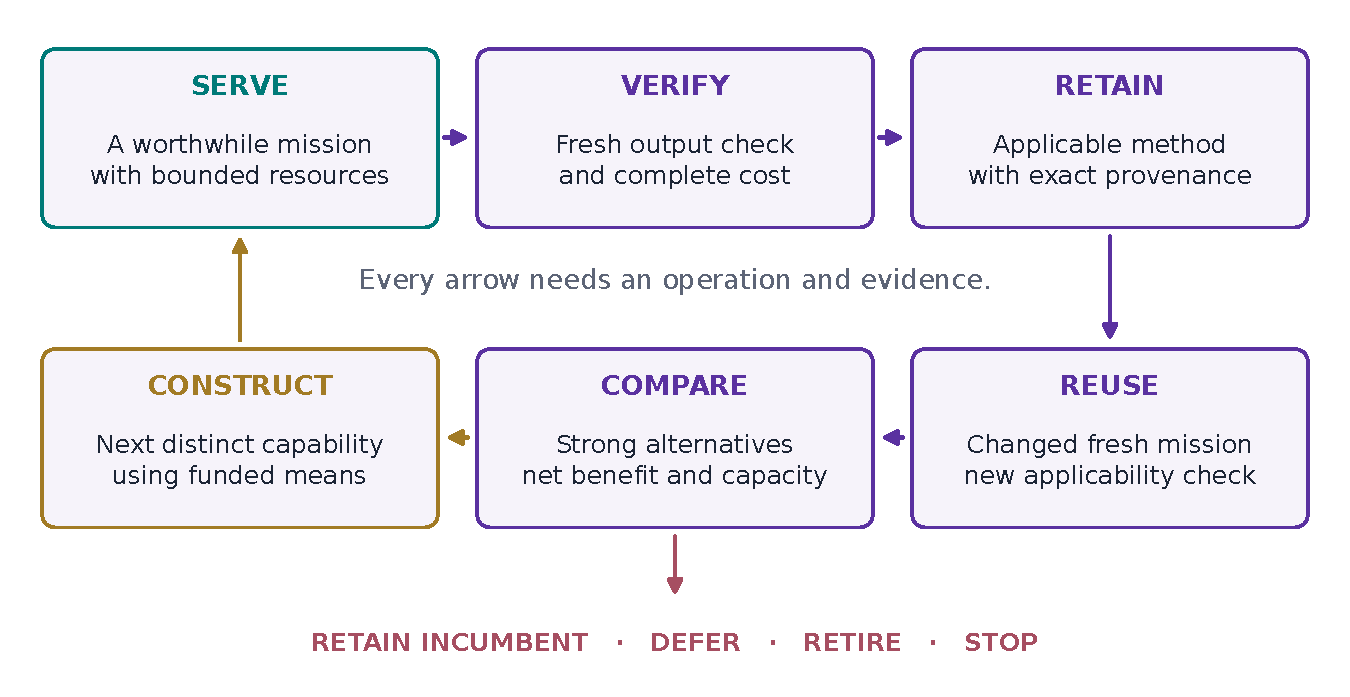
\includegraphics[width=\linewidth]{figures/mission-capability-loop.pdf}
\caption{The obligation at each turn. A checked useful result supplies evidence and a candidate method. Reuse and
successor construction remain subject to independent output checks and separate cost decisions.}
\label{fig:loop}
\end{figure}

\subsection{Reconcile the failure before changing the experiment}

A read-only audit rechecks 96 primary checkpoints, 48 diagnostic checkpoints, twelve diagnostic raw archives
and all 52 files in the earlier freeze. At each primary acquisition stage, a 500,000-unit ceiling protected
401,024 units for qualification: 80.20\% of the budget. Search had at most 98,976 units before other control
reserves. The eight-method successive-halving race required up to seventeen paid calls to finish six training
cases, but every primary stream stopped after eleven to thirteen calls. All 140 paid prefixes were valid and
untruncated. Twelve subsequent calls were refused before computation. Qualification and admission were never reached.

Of 96 menu entries, 58 were ordinary eliminations, 26 were incomplete valid prefixes, and twelve were unfunded
calls. Reserved qualification allowance was not spent work. Raising the overall stream budget to two million
units left this acquisition ceiling unchanged. Marking a stage completed before acquisition also made that
failure terminal; later stages deferred without an accepted parent.

The prior cost model additionally charged 5,238,180 units to checkpoint rewriting, 44.7\% of primary flywheel
work. Research and service shared a cumulative account. These observations support an allocation mismatch,
expensive persistence and weak isolation of promised delivery. They do not demonstrate a corrupt numerical
result or prove that no transferable scheduling method exists. The diagnostic nevertheless warns against treating
allocation repair as sufficient: inherited work averaged 888,009.50 units for 36 qualified outputs across 48
requests, while the parent-removed conventional alternative averaged 225,339.33 and qualified 37.

The earlier package also recovered SUCCESSOR $\Omega$---Strategy Laboratory v0.1.0, archive SHA-256 beginning
\artifact{c0df2ac39ddcb32d}, and replayed its unchanged frozen policies under CPython 3.13.5. All six attempts
and 27,648 cases reproduced their non-timing outputs and judgments; a separate artifact audit checked
193,536 policy/control artifacts. This verified historical replay did not rerun acquisition search, establish
equal total computation against specialists, or qualify the present flywheel. The full historical evidence
remains in the prior edition; byte-bound status and replay records are copied into this edition's audit docket.

The new study therefore changes the domain, construction representation, accounting, causal predecessor,
persistence and comparators. It uses new identities and new tasks. The earlier evidence is an audited motivation,
not a reused confirmation set.

\subsection{An operational interpretation of the Out stages}

\begin{table}[htbp]\centering\small
\begin{tabularx}{\linewidth}{@{}L{27mm}Y@{}}\toprule
Stage & Inspectable operation and evidence \\\midrule
Identify & Bounded three-domain screen; fixed mission stream and explicit scope. \\
Out-Learn & Accepted response, edge checker, development cost table and retained regression counterexamples. \\
Out-Think & Compare low-rank construction with native refactorization using a frozen forecast. \\
Out-Design & Construct factor or update arrays with a typed interface, operator identity and dependencies. \\
Out-Strategise & Reserve service, research or released quota; defer when allowance or scope is insufficient. \\
Out-Execute & Original workbench dispatch, native computation, independent numerical check and exact receipt. \\
Out-Evolve & Retain scoped instruments, reject stale reuse, preserve the incumbent and select the next permitted request. \\\bottomrule
\end{tabularx}
\caption{An implementation role for the conceptual stages. These names do not imply seven independent models or
an unconstrained discovery process. The frozen methods and data are the operative mechanism.}
\end{table}
